\subsection{Virtual Displacements and the Birth of the Euler-Lagrange Equation}

This led him into the territory of what we now call \textbf{variational calculus} — a kind of calculus where the unknowns are not just numbers or functions, but entire paths and trajectories. It was here that Lagrange made his most profound contribution: a symbolic recipe to determine the true path of motion, not by tracing it directly, but by ruling out all the alternatives.


\medskip

\begin{HistoricalSidebar}{Lagrange and the Calculus of the Best Possible World}
    
        \textbf{Gottfried Wilhelm Leibniz} (1646–1716) believed that the universe was a rational, optimized system—created by a perfect God who chose the \textbf{best of all possible worlds}. For Leibniz, this meant that nature always followed the most elegant, efficient paths. Every event had a sufficient reason, and every motion unfolded with mathematical necessity.
    
        \medskip
    
        This vision wasn’t just theological—it was mathematical. Leibniz imagined a cosmos that could be described in terms of \textbf{infinitesimals, differentials, and minima}, governed by the principle that nature “does nothing in vain.” These ideas laid the philosophical and technical groundwork for the development of calculus, and they would find their purest mechanical expression in the work of \textbf{Joseph-Louis Lagrange}.
    
        \medskip
    
        In his 1788 masterpiece, \textit{Mécanique Analytique}, Lagrange reformulated Newtonian mechanics using only algebra and calculus, eliminating the need for geometric diagrams or direct references to physical forces. Instead, he treated the evolution of physical systems as an \textbf{optimization problem}—exactly the kind of principle Leibniz had championed.
    
        \medskip
    
        Lagrange’s use of the \textbf{principle of least action}—that nature selects the path which minimizes (or extremizes) a certain quantity—was a direct echo of Leibniz’s metaphysics. In Lagrange’s mechanics, the universe behaves not like a machine of levers and weights, but like a system solving an elegant equation: \textbf{minimal effort, maximal coherence}.
    
        \medskip
    
        \textbf{Quote from Leibniz (1697):}
        \begin{quote}
        “In the effects of nature, the greatest variety is brought about with the greatest order; and this is the mark of divine wisdom.”
        \end{quote}
    
        Leibniz dreamed of a universe governed by calculus. Lagrange wrote the equations that made it move.
    
\end{HistoricalSidebar}

\medskip

The idea of a \textit{virtual displacement} predates Lagrange, going back to the principle of \textit{virtual work} used by early mechanicians like Galileo, Torricelli, and the Bernoulli brothers. These were imagined shifts—not real motions—tiny hypothetical nudges you could apply to a system in equilibrium to see how the forces would respond.

Lagrange took that idea and breathed motion into it.

He reinterpreted these imaginary displacements as probes—not of static balance, but of dynamic possibility. What if, he asked, we could apply a small tweak — not to the forces, but to the \textit{path itself}? What if nature picks the path where these imagined variations make no first-order difference?

\subsubsection{Stationarity: The Vanishing of First‐Order Variation}

To say that a virtual tweak in the path makes “no first‐order difference” is to demand that the linear term in the change of some quantity vanishes.  In Lagrange’s language, if \(S[q]\) is the action functional (the time‐integral of the Lagrangian), and we deform the path \(q(t)\) by a small virtual displacement \(\delta q(t)\), then

\[
\Delta S \;=\; S[q + \delta q] - S[q]
\;=\; \underbrace{\int \frac{\delta S}{\delta q}\,\delta q\,dt}_{\text{first‐order}} + \mathcal{O}(\delta q^2).
\]

Requiring “no first‐order difference” means
\[
\int \frac{\delta S}{\delta q}\,\delta q\,dt = 0
\quad\Longrightarrow\quad
\frac{\delta S}{\delta q} = 0
\]
for every admissible \(\delta q\).  In other words, the first‐order (linear) variation vanishes, so any residual change in \(S\) is at least second order in the small displacement.


\subsubsection{Second‐Order Smallness: Beyond the Stationary Point}

Once the first‐order (linear) term in the variation vanishes, the remaining change in the action is at least of order \(\delta q^2\).  Concretely, if we expand

\[
\Delta S = S[q + \delta q] - S[q]
= \underbrace{\int \frac{\delta S}{\delta q}\,\delta q\,dt}_{=0}
+ \tfrac12 \iint \frac{\delta^2 S}{\delta q(t)\,\delta q(t')}\,\delta q(t)\,\delta q(t')\,dt\,dt'
+ \mathcal{O}\bigl(\|\delta q\|^3\bigr),
\]

then “at least second order” means

\[
\Delta S = \mathcal{O}\bigl(\|\delta q\|^2\bigr).
\]

In practical terms:
\begin{itemize}
  \item If you halve the size of your virtual displacement, the residual change in \(S\) drops by a factor of four (or more).
  \item The action surface is “flat” to first order, so nearby paths differ only by these much smaller, quadratic‐scale corrections.
  \item This quadratic dominance guarantees that the chosen path is not merely stationary but a \emph{local extremum} (minimum, maximum, or saddle point) of the action.
\end{itemize}

Physically, it means that small wiggles around the true trajectory do not change the action significantly—only when you make a finite (non‐infinitesimal) deviation does the action differ appreciably.  Thus Lagrange’s criterion of “no first‐order difference” secures the dynamical path as the one for which the action is extremal, with any departure penalized only at second order or higher.  


\subsubsection{Physical interpretation:}  
A system “chooses” the path for which the action is stationary—neither increasing nor decreasing to first order under any infinitesimal variation.  This stationarity condition directly yields the Euler–Lagrange equations, the dynamical equations of motion in Lagrange’s formulation:

\[
\frac{d}{dt}\!\bigl(\partial_{\dot q}L\bigr)
\;-\;\partial_{q}L
\;=\;
0.
\]

Thus, “no first‐order difference” transforms the ancient idea of virtual work into a powerful variational principle governing dynamics.  



\medskip

\begin{HistoricalSidebar}{The Principle of Virtual Work}
  Long before the age of Lagrange, mechanicians had recognized that you could probe a system’s balance by 
  imagining “infinitesimal” shifts.  In the early 17\textsuperscript{th} century, Galileo—while studying 
  the lever—implicitly used virtual displacements to compare weights and distances.  Evangelista Torricelli 
  and the Bernoulli brothers (particularly Johann and Jakob) extended the idea to fluids and elastic 
  systems, noting that an imagined nudge at equilibrium yields no net “virtual work.”  

  \medskip

  Lagrange would later embrace this dynamic virtual work, recasting it into his variational calculus and 
  showing that the true path makes the \emph{action} stationary.  Thus, what began as a static balancing 
  trick became the cornerstone of analytical mechanics.
\end{HistoricalSidebar}



\subsection{Emergence of Kinetic and Potential Energy from Variational Principles}

Having seen that “no first‐order difference” in the action picks out the true path, we can now ask: what form must the action take so that the resulting Euler–Lagrange equations reproduce the familiar Newtonian dynamics?  The answer leads naturally to the concepts of kinetic and potential energy.

\medskip

\noindent\textbf{Generalized virtual work.}  Recall that a generalized force \(Q_{i}\) does virtual work
\[
\delta W = \sum_{i} Q_{i}\,\delta q_{i}.
\]
If these forces are conservative, there exists a scalar function \(V(q)\) (the potential energy) such that
\[
Q_{i} = -\frac{\partial V}{\partial q_{i}}
\quad\Longrightarrow\quad
\delta W = -\sum_{i} \frac{\partial V}{\partial q_{i}}\,\delta q_{i}
= -\,\delta V.
\]

\medskip

\noindent\textbf{Kinetic energy from the momentum term.}  On the other hand, the Euler–Lagrange equations arise from
\[
\frac{d}{dt}\!\bigl(\partial_{\dot q_{i}}L\bigr) - \partial_{q_{i}}L = 0.
\]
To reproduce Newton’s second law \(m\ddot q_{i} = Q_{i}\), one identifies
\[
\partial_{\dot q_{i}}L = m\,\dot q_{i}
\quad\Longrightarrow\quad
L \supset \tfrac12\,m\,\dot q_{i}^{2}.
\]
Thus the \emph{kinetic energy} emerges as the quadratic form
\[
T = \tfrac12 \sum_{i} m\,\dot q_{i}^{2}.
\]

\medskip

\noindent\textbf{The full Lagrangian and equations of motion.}  Combining kinetic and potential contributions into the Lagrangian
\[
L(q,\dot q) = T(\dot q) - V(q),
\]
the Euler–Lagrange equations become
\[
\frac{d}{dt}\!\bigl(m\,\dot q_{i}\bigr)
- \bigl(-\tfrac{\partial V}{\partial q_{i}}\bigr)
= 0
\quad\Longrightarrow\quad
m\,\ddot q_{i} = -\frac{\partial V}{\partial q_{i}},
\]
exactly Newton’s law \(m\ddot q_{i}=Q_{i}\) with \(Q_{i}=-\partial_{q_{i}}V\).

\medskip

\noindent\textbf{Intuitive takeaway.}  In Lagrange’s variational framework:

\begin{itemize}
  \item The \emph{momentum} \(p_{i} = \partial_{\dot q_{i}}L\) leads directly to the identification \(p_{i}=m\dot q_{i}\).  
  \item The \emph{kinetic energy} \(T\) is the natural quadratic function of these momenta (or velocities).  
  \item A \emph{conservative force} derives from a potential \(V(q)\), with virtual work \(\delta W=-\delta V\).  
  \item The combination \(L = T - V\) guarantees that extremizing the action enforces both inertia (\(m\ddot q\)) and conservative forces in one unified algebraic step.
\end{itemize}

Thus kinetic and potential energy are not ad hoc additions, but the inevitable ingredients of any action principle whose stationarity reproduces the familiar Newtonian dynamics.  



\subsection{The Spirit of Determinism}

The Lagrangian method captured the Enlightenment dream: a physics of perfect predictability. Every system, no matter how complex, could be described not by what happens, but by what \textit{must} happen, according to laws derived from symmetry, structure, and principle.

Where Newton saw objects being pushed and pulled, Lagrange saw trajectories preordained by the internal logic of energy. It was a vision of the cosmos as a deterministic scroll, already written — with the Euler-Lagrange equation as its grammar.

\begin{quote}
    \textit{Nature explores all the paths it could take — and chooses the one where the story is already most coherent.}
\end{quote}


\begin{HistoricalSidebar}{Fermat and the Wisdom of Light}

    In the 1600s, while Descartes was busy mathematizing the heavens and Galileo was redefining motion, \textbf{Pierre de Fermat} made a deceptively simple observation about something far less massive: \emph{light}.

    \medskip
    
    Fermat proposed what would become known as the \textbf{Principle of Least Time}: \emph{light always travels between two points along the path that takes the least time}. It wasn’t just a guess—it matched experimental results, especially the strange bending of light as it passed from air into water.

    \medskip
    
    While Descartes had explained refraction using the force of impact, Fermat took a different route. He calculated the path a light ray would take if it "chose" the fastest route—slower in water, faster in air—and astonishingly, this mathematical minimum exactly matched what nature actually did.

    \medskip
    
    In other words, Fermat believed the universe was lazy in a profoundly elegant way: it always optimized.
    
    \medskip
    
    A century later, \textbf{Joseph-Louis Lagrange} would elevate this idea into a new language entirely: the \textbf{calculus of variations}. Instead of just light, Lagrange applied it to the motion of \emph{everything}. Why do planets move the way they do? Because their paths make the action minimal. Why does a pendulum swing the way it does? Same reason. Just as Fermat’s light found the quickest path, Lagrange’s mechanics found the most efficient one—mathematically encoded as the path that extremizes a function called the \textit{Lagrangian}.

    \medskip
    
    Thus, Fermat’s humble ray of light cast a long shadow—one that reached all the way into the foundations of modern physics.
    
\end{HistoricalSidebar}

   





\subsection{Generalized Coordinates in Lagrange’s Mechanics}

Lagrange showed that for a system with \(n\) independent variables \(q_1,\dots,q_n\), one may regard the Lagrangian as a function of the coordinates, their time-rates, and time itself:
\[
L \;=\; L\bigl(q_1,\dots,q_n,\;q_1',\dots,q_n',\;t\bigr),
\]
where \(q_i'=\tfrac{dq_i}{dt}\).  He then used the notation
\[
\frac{dL}{dq_i}
\quad\text{and}\quad
\frac{dL}{dq_i'},
\]
to mean “how \(L\) changes when \(q_i\) alone is varied” and “how \(L\) changes when \(q_i'\) alone is varied,” holding all other \(q_k\) and \(q_k'\) constant.

Applying his variational recipe to each coordinate \(q_i\), Lagrange arrived at a set of \(n\) equations of motion, one for each \(i=1,\dots,n\):
\[
\frac{d}{dt}\!\Bigl(\frac{dL}{dq_i'}\Bigr)
\;-\;
\frac{dL}{dq_i}
\;=\;
0.
\]
With this compact algebraic rule, he replaced the old Cartesian force-balance methods by a unified system of equations—without ever invoking partial derivatives or modern manifold concepts.  



\subsection{Lagrange’s Coordinate–Velocity Space}

Rather than work solely with positions or forces, Lagrange treated each instantaneous state of a system as a point in a “coordinate–velocity space.”  For a system with \(n\) degrees of freedom, one records
\[
\bigl(q_1,\dots,q_n;\;q_1',\dots,q_n'\bigr),
\]
where \(q_i\) is the generalized coordinate and \(q_i'=\tfrac{dq_i}{dt}\) its time‐rate.  This \(2n\)-tuple uniquely fixes both where the system is and how it is moving.

\medskip

On this space Lagrange defined his function
\[
L\bigl(q_1,\dots,q_n;\;q_1',\dots,q_n';\;t\bigr)
\;=\;
T-V,
\]
assigning to each point the difference of kinetic and potential energy.  A motion of the system then becomes a curve
\[
t\;\longmapsto\;\bigl(q_i(t),\,q_i'(t)\bigr)
\]
in this space, and the true motion is singled out by the requirement that the integral of \(L\) along the curve be stationary.

\medskip

Viewed in this way, Lagrange’s method unifies position and velocity into one arena: every equation of motion emerges from the single variational principle applied to \(L\) on the full coordinate–velocity space.  


\begin{figure}[H]
    \centering
    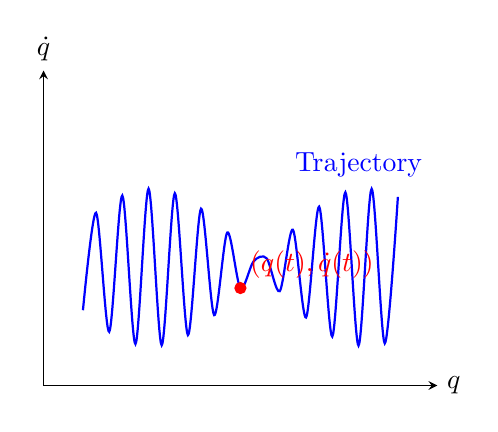
\begin{tikzpicture}[>=stealth, scale=1]
      % Axes
      \draw[->] (0,0) -- (5,0) node[right] {$q$};
      \draw[->] (0,0) -- (0,4) node[above] {$\dot q$};
      % Trajectory curve
      \draw[thick, domain=0.5:4.5, smooth, variable=\t, blue]
        plot ({\t}, {1.5 + 1*sin(20*\t r)});
      % Mark a point on the trajectory
      \coordinate (P) at (2.5,{1.5 + sin(20*2.5 r)});
      \filldraw[red] (P) circle (2pt)
        node[above right] {$(q(t),\dot q(t))$};
      % Label the curve
      \node[blue] at (4,2.8) {Trajectory};
    \end{tikzpicture}
    \caption{Illustration of a curve in Lagrange’s coordinate–velocity space for a single degree of freedom.}
\end{figure}




\subsection{Kepler’s Second Law in \emph{(r,\(\theta\))} Configuration Space}

In Lagrange’s formulation, the motion of a planet under a central force can be viewed as a path in the two-dimensional configuration space with coordinates \((r,\theta)\).  The Lagrangian for a mass \(m\) orbiting a central body of mass \(M\) is

\[
L(r,\dot r,\dot\theta)
=\tfrac12\,m\bigl(\dot r^2 + r^2\dot\theta^2\bigr)
\;+\;\frac{G\,M\,m}{r},
\]

and since \(\theta\) does not appear explicitly in \(L\), the corresponding “generalized momentum”

\[
p_\theta \;=\; \frac{dL}{d\dot\theta} \;=\; m\,r^2\,\dot\theta
\]

is conserved.  But geometrically \(r^2\dot\theta\) is twice the areal velocity \(dA/dt\), so

\[
r^2\,\dot\theta \;=\;\text{constant}
\quad\Longrightarrow\quad
\frac{dA}{dt}=\tfrac12\,r^2\dot\theta=\text{constant},
\]

which is exactly Kepler’s Second Law: \emph{equal areas in equal times}.  

\begin{figure}[H]
\centering
\begin{tikzpicture}[>=stealth, xscale=0.02, yscale=1]
  % Axes
  \draw[->] (0,0) -- (370,0) node[right] {$\theta$ (deg)};
  \draw[->] (0,0) -- (0,4) node[above] {$r(\theta)$};
  % Elliptical orbit in (r,theta) space: r = a(1−e²)/(1+e cos θ), here a=3, e=0.5
  \draw[thick,domain=0:360,smooth,samples=200,blue]
    plot (\x,{2.25/(1+0.5*cos(\x))});
  % Mark aphelion and perihelion
  \filldraw[red] (180,{2.25/(1+0.5*cos(180))}) circle (2pt)
    node[above right] {aphelion};
  \filldraw[red] (0,{2.25/(1+0.5*cos(0))}) circle (2pt)
    node[below right] {perihelion};
  % Label curve
  \node[blue] at (200,3.2) {$(r(\theta),\theta)$};
\end{tikzpicture}
\caption{An elliptical orbit represented as a curve in the \((r,\theta)\) configuration space, where \(r(\theta)=\tfrac{a(1-e^2)}{1+e\cos\theta}\).}
\end{figure}



\begin{figure}[H]
    \centering
    % First (Cartesian) illustration
    \subcaptionbox{Ellipse in Cartesian $(x,y)$ plane\label{fig:ellipse-cartesian}}{%
      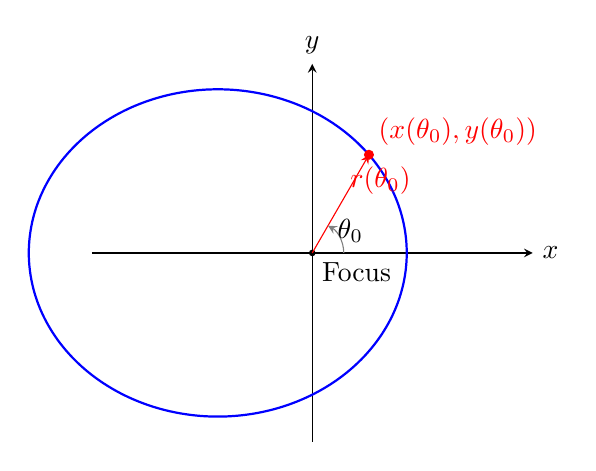
\begin{tikzpicture}[>=stealth,scale=0.8]
        % Axes
        \draw[->] (-3.5,0) -- (3.5,0) node[right] {$x$};
        \draw[->] (0,-3) -- (0,3) node[above] {$y$};
        % Elliptical orbit
        \draw[thick,blue,domain=0:360,smooth,samples=200]
          plot ({(2.25/(1+0.5*cos(\x)))*cos(\x)},
               {(2.25/(1+0.5*cos(\x)))*sin(\x)});
        % Focus
        \fill (0,0) circle (1.5pt) node[below right] {Focus};
        % Sample point at θ₀=60°
        \coordinate (P) at ({1.8*cos(60)},{1.8*sin(60)});
        \filldraw[red] (P) circle (2pt) node[above right] {$(x(\theta_0),y(\theta_0))$};
        % Radius vector
        \draw[red,->] (0,0) -- (P) node[midway,above right] {$r(\theta_0)$};
        % Angle arc
        \draw[->,gray] (0.5,0) arc[start angle=0,end angle=60,radius=0.5];
        \node at ({0.7*cos(30)},{0.7*sin(30)}) {$\theta_0$};
      \end{tikzpicture}
    }
    
    \vspace{1em}
    
    % Second (configuration‐space) illustration
    \subcaptionbox{Configuration‐space plot $r$ vs.\ $\theta$\label{fig:ellipse-rt}}{%
      \begin{tikzpicture}[>=stealth,xscale=0.02,yscale=1]
        % Axes
        \draw[->] (0,0) -- (370,0) node[right] {$\theta$ (deg)};
        \draw[->] (0,0) -- (0,4)   node[above] {$r(\theta)$};
        % r(θ) curve
        \draw[thick,blue,domain=0:360,smooth,samples=200]
          plot (\x,{2.25/(1+0.5*cos(\x))});
        % Sample point at (60,1.8)
        \filldraw[red] (60,1.8) circle (2pt) node[above right] {$(\theta_0,r(\theta_0))$};
        % Guides
        \draw[gray,dashed] (60,0) -- (60,1.8) -- (0,1.8);
      \end{tikzpicture}
    }
    
    \caption[Cartesian and $(r,\theta)$ views of an ellipse]{%
    Left: the physical orbit in the $(x,y)$ plane, drawn from the focus at the origin, with a sample radius vector $r(\theta_0)$.  
    Right: the corresponding curve in $(r,\theta)$ configuration space, showing how the same angle $\theta_0$ maps to the radial distance $r(\theta_0)$.}
\end{figure}
    